\chapter{Dataverzameling}
\label{ch:dataverzameling}

Voor deze studie werden meerdere videofragmenten verzameld van drie fundamentele krachtoefeningen: de \textbf{Bench Press}, \textbf{Deadlift} en \textbf{Squat}. 
Elk videofragment werd opgenomen van de \textbf{rechterzijde} van het lichaam van de sporter, zodat de volledige beweging van de rechterkant zichtbaar is tijdens de uitvoering. 
De opnames zijn gemaakt onder gecontroleerde omstandigheden en met een constante camerahoek om uniforme gegevens te waarborgen.

Voor elke oefencategorie zijn zowel correcte als foutieve uitvoeringen geregistreerd. 
De foutieve uitvoeringen werden systematisch gecategoriseerd op basis van biomechanische afwijkingen die visueel detecteerbaar zijn. 
Hieronder worden per oefening de verschillende types afwijkingen beschreven, inclusief de relevante hoeken tussen deze keypoints.

\section{Bench Press}

\subsection*{Correcte Uitvoeringen}
Meerdere correcte uitvoeringen zijn opgenomen waarbij de barbell gecontroleerd naar de borst wordt gebracht en teruggeduwd met een neutrale polspositie, stabiele schouderpositie en volledige \textit{range of motion} (ROM).

\begin{figure}[h]
    \centering
    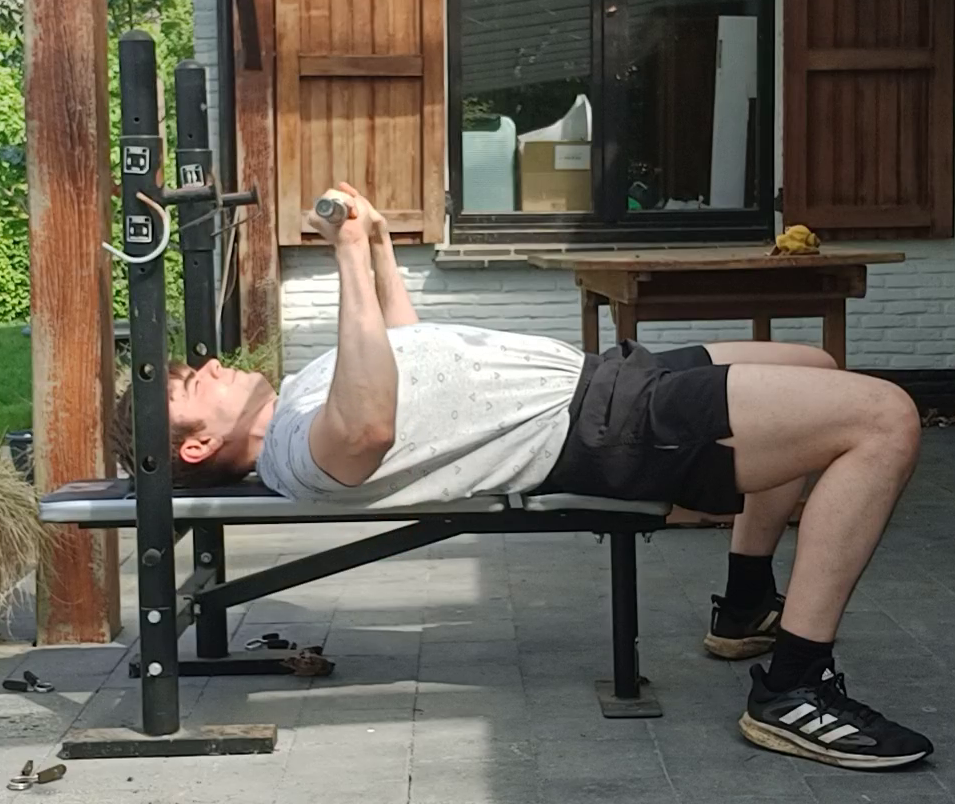
\includegraphics[width=0.5\textwidth]{bench_press_correct.png}
    \caption{Correcte uitvoering van Bench Press (zijaanzicht)}
    \label{fig:bench_correct}
\end{figure}

\subsection{Foutieve Uitvoeringen}
\begin{itemize}
    \item \textbf{Ellebogen te hoog:} Hoek tussen \textit{elleboog–schouder–pols} benadert 180°, wat wijst op een overdreven horizontale armpositie.
    
    \begin{figure}[h]
        \centering
        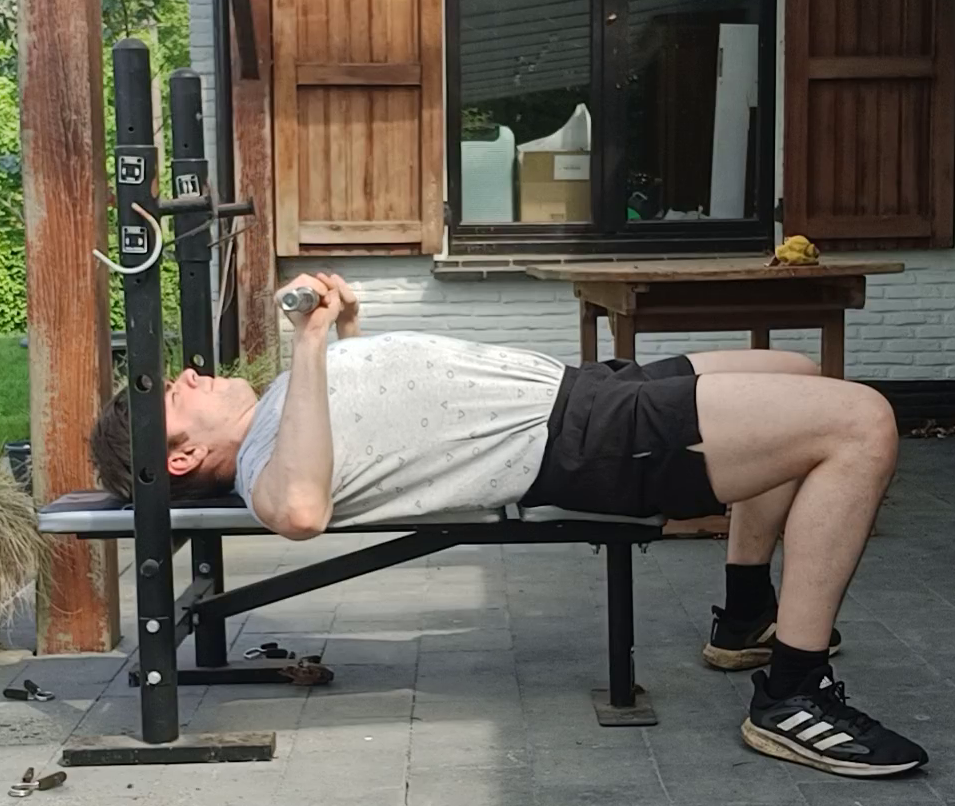
\includegraphics[width=0.5\textwidth]{bench_elbows_high.png}
        \caption{Bench Press met te hoge ellebogen}
        \label{fig:bench_elbows_high}
    \end{figure}
    
    \item \textbf{Te smalle handgreep:} Hoek tussen \textit{ellebogen t.o.v. schouderlijn} is kleiner dan 90°.
    
    \begin{figure}[h]
        \centering
        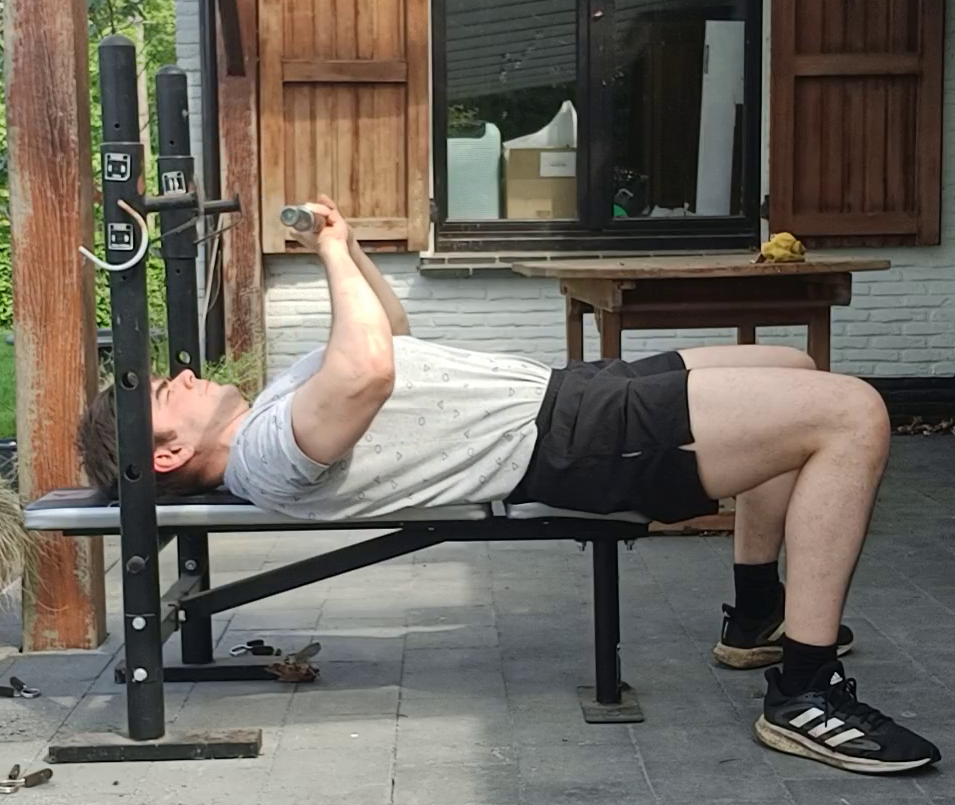
\includegraphics[width=0.5\textwidth]{bench_narrow_grip.png}
        \caption{Bench Press met te smalle handgreep}
        \label{fig:bench_narrow_grip}
    \end{figure}
    
    \item \textbf{Onvolledige herhaling:} Barbell raakt de borst niet; hoek tussen \textit{elleboog–schouder–heup} blijft groter dan 90°.
    
    \item \textbf{Gestrekte knieën:} Hoek tussen \textit{heup–knie–enkel} benadert 180°.
    
    \item \textbf{Pelvis niet op bank:} Afstand tussen heup en bank toont loskomen; hoek \textit{heup–schouder–knie} > 150°.
\end{itemize}

\section{Deadlift}

\subsection{Correcte Uitvoeringen}
De correcte uitvoeringen tonen een rechte rug, neutrale hoofdpositie, stabiele heup-knie-analyse en een verticale barbellbeweging.

\begin{figure}[h]
    \centering
    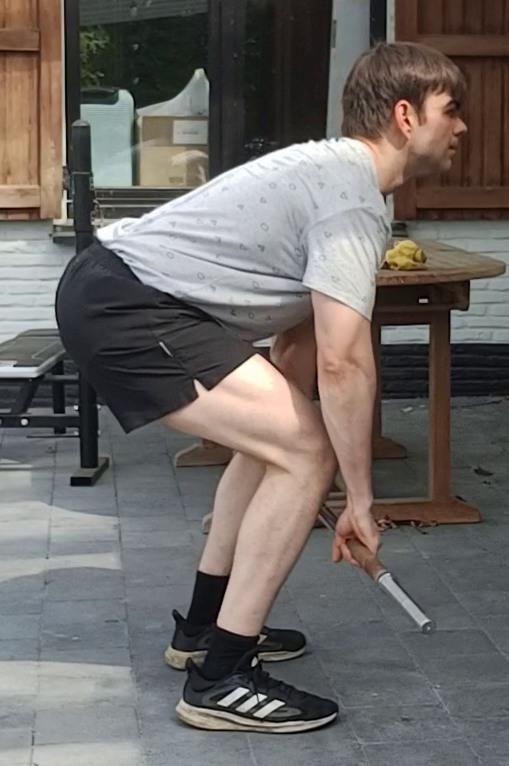
\includegraphics[width=0.5\textwidth]{deadlift_correct.png}
    \caption{Correcte uitvoering van Deadlift}
    \label{fig:deadlift_correct}
\end{figure}

\subsection{Foutieve Uitvoeringen}
\begin{itemize}
    \item \textbf{Kromme rug:} Hoek \textit{schouder–heup–knie} < 160°.
    
    \item \textbf{Te smalle handgreep:} Hoek \textit{elleboog–schouder–elleboog (frontaal)} < 50°.
    
    \item \textbf{Onvolledige herhaling:} Hoek \textit{heup–knie–enkel} blijft > 160°; \textit{schouder–heup–knie} < 180°.
    
    \item \textbf{Te smalle voetstand:} Enkelafstand < heupbreedte; hoek \textit{heup–knie–enkel} vaak < 90°.
    
    \item \textbf{Te brede voetstand:} Enkelafstand > schouderbreedte; resulteert in beperkte ROM.
    
    \item \textbf{Voorover leunen:} Hoek \textit{schouder–heup–enkel} wijkt > 10° af van de verticale as.
\end{itemize}

\begin{figure}[h]
    \centering
    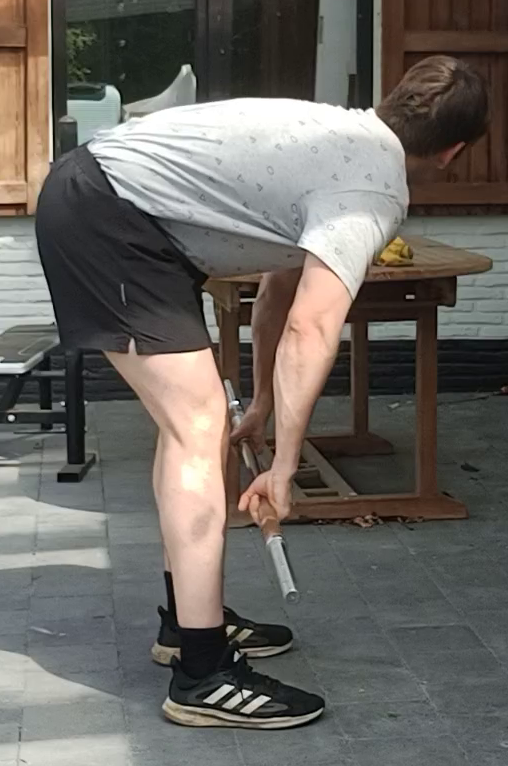
\includegraphics[width=0.5\textwidth]{deadlift_rounded_back.png}
    \caption{Deadlift met kromme rug}
    \label{fig:deadlift_rounded_back}
\end{figure}

\section{Squat}

\subsection{Correcte Uitvoeringen}
De correcte squats tonen diepe bewegingen tot onder parallel, rechte rug en stabiele knie- en enkelpositionering.

\begin{figure}[h]
    \centering
    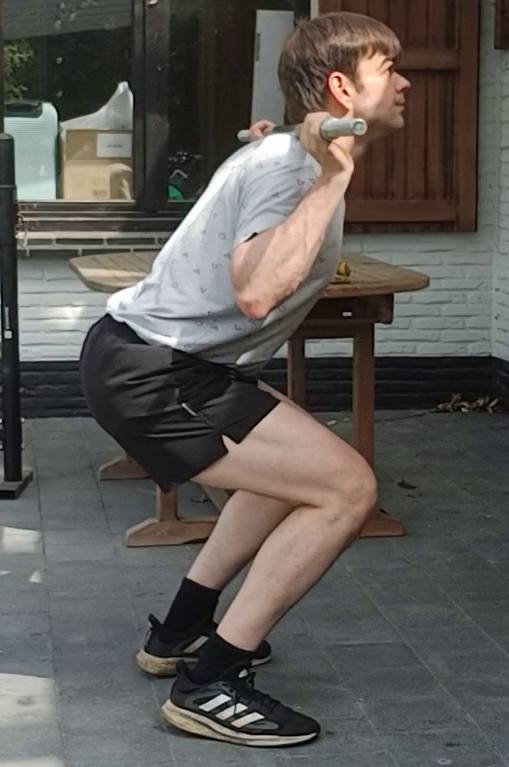
\includegraphics[width=0.5\textwidth]{squat_correct.png}
    \caption{Correcte uitvoering van Squat}
    \label{fig:squat_correct}
\end{figure}

\subsection{Foutieve Uitvoeringen}
\begin{itemize}
    \item \textbf{Kromme rug:} Hoek \textit{schouder–heup–knie} < 160°.
    
    \item \textbf{Onvolledige herhaling:} Hoek \textit{heup–knie–enkel} > 100°, geen diepe squat.
    
    \item \textbf{Te brede voetstand:} Enkelafstand overschrijdt schouderbreedte; hoek \textit{knie–enkel–tenen} > 30°.
\end{itemize}

\begin{figure}[h]
    \centering
    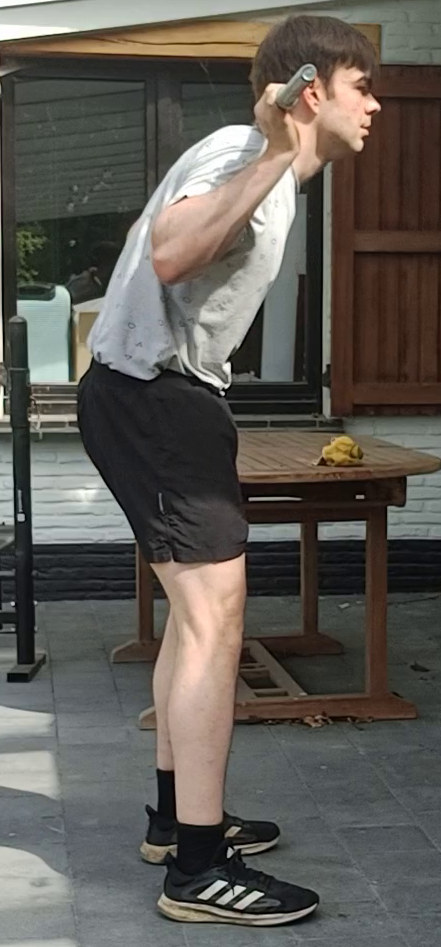
\includegraphics[width=0.5\textwidth]{squat_rounded_back.png}
    \caption{Squat met kromme rug}
    \label{fig:squat_rounded_back}
\end{figure}

\section{Conclusie}
Alle fragmenten zijn zorgvuldig geselecteerd en gecategoriseerd om een evenwichtige dataset te vormen met zowel correcte als incorrecte bewegingspatronen. 
